\chapter{Úvod do problematiky testování materiálů, metody vlastního testování, metoda akustické emise}

\section{Nedestruktivní testování}
V technické praxi jsou struktury namáhány mnoha vnějšími vlivy, čímž se mění jejich materiálové vlastnosti. Například, u laminátových kontrukcí v leteckém průmyslu může vlivem sil nárazu pevnost v tlaku klesnout až o 80\%, i když se materiál jeví jako nepoškozený \cite{Benes_podklad_advances}. 

Pro posouzení stavu materiálu je proto nutné provádět pravidelné testování.
Za účelem stanovení mezních vlastností materiálu jako pevnosti v tlaku, pevnosti v~tahu, lomové houževnatosti, atd., bývá prováděno \ac{DT}. Zahrnuje např. zkoušku tahem, tlakem, nebo ohybem. K těmto zkouškám jsou používány speciální stroje – kladiva, trhačky, ohýbačky, aj. Jak je z názvu přímo patrné, vlastní destruktivní zkoušení končí nevratným poškozením vzorku. 

Pro již hotové konstrukce (např. svařované konstrukce v zámečnické výrobě, betonové pilíře v oblasti stavebnictví) nebo komponenty (hřídele, ozubená kola, kolejnice, atd.) se metody \ac{DT} zpravidla nepoužívají, jelikož by takové zkoušení bylo příliš nákladné. Nabízí se proto použití metod \ac{NDT}. Počátky \ac{NDT} sahají do 19. století, kdy pomocí tzv. akustického poklepového testování byly detekovány praskliny na železničních kolech \cite{ConcretetestingHELAL}.
\section{Metody nedestruktivního testování}
Velká výhoda metod \ac{NDT} spočívá v možnosti zkoušení v kterékoliv části životního cyklu produktu, u některých metod dokonce i v průběhu vykonávání vlastní činnosti výrobku. Díky tomu dostáváme přesné informace o poloze a závažnosti případného defektu ve struktuře materiálu. V současné době na trhu dominuje pět metod nedestruktivního testování – zkoušení magnetickými částicemi, radiografické zkoušení, ultrazvukové zkoušení, zkoušení vířivými proudy a zkoušení metodou akustické emise (dále AE).

Zkoušení magnetickými částicemi spočívá ve vystavení feromagnetických materiálů magnetickému poli. Díky vysoké permeabilitě feromagnetického materiálu se magnetické domény orientují ve~směru působení magnetického pole, tvoří tak souvislé čáry. V případě nespojitosti materiálu dojde k tzv. úniku magnetického pole – čáry v~bodě defektu nebudou spojité. Pro~snadnou viditelnost těchto nespojitostí je použit prášek oxidu železitého, který zmíněné čáry a nespojitosti kopíruje \cite{Gupta_ADVANCES_IN_MATERIALS_AND_PROCESSING_TECHNOLOGIES}. Mezi~limity spadá možnost použití jen pro feromagnetické materiály (železo, kobalt, nikl, ferity, gadolinium, aj.) \cite{Sandeep_Kumar_Dwivedi_NDT}.

Radiografické zkoušení je postup založen na snímání obrázků s využitím radioaktivního zdroje záření. Záření je pohlcováno materiálem a dochází tak k útlumu. Defekty na těchto snímcích lze rozpoznat jako místa s menším útlumem záření \cite{Gupta_ADVANCES_IN_MATERIALS_AND_PROCESSING_TECHNOLOGIES}. Limity představuje nutnost radiační ochrany a nevhodnost použití pro porézní materiály (např. beton, dřevo, sádra, keramiky, kosti aj.) \cite{Sandeep_Kumar_Dwivedi_NDT}

Při zkoušení ultrazvukem je používáno zvukových vln. Piezoelektrický snímač generuje pulzy, které se šíří materiálem. Cestují-li tyto pulzy nepoškozenou, spojitou strukturou, nemění se jejich parametry (především tedy rychlost). Při defektu dochází ke změně rychlosti pulzů.\cite{Gupta_ADVANCES_IN_MATERIALS_AND_PROCESSING_TECHNOLOGIES}. 

Během zkoušení vířivými proudy je kovový materiál umístěn do fluktuujího magnetického pole, které je vytvářeno cívkou. V kovovém materiálu jsou indukovány proudy s vířivou povahou (proto vířivé proudy). Těmito vířivými proudy je vytvořeno sekundární magnetické pole, které ovlivňuje pole cívky. S defektem ve struktuře materiálu dojde tedy ke změně i vířivých proudů, což ovlivní i primární magnetické pole cívky \cite{Gupta_ADVANCES_IN_MATERIALS_AND_PROCESSING_TECHNOLOGIES}. 
\section{Metoda AE. Její výhody, limity}
V případě, že je kovový materiál deformován, uvolňuje se energie ve formě tzv. elastických vln. Tyto elastické vlny jsou vlny vysoké frekvence, které cestují směrem k~povrchu materiálu. Na povrchu tato data sbírají snímače AE. Souřadnice zdrojů AE jsou nejčastěji stanovovány pomocí známého triangulačního algoritmu (podle normy ČSN 14584 \cite{čsn14584}) dle časových diferencí příchodů signálů k jednotlivým snímačům. Tyto snímače jsou na zkoušeném vzorku umístěny v husté síti.

Oproti ultrazvukovému testování je velkou výhodou zkoušení AE možnost nepřetržitého monitorování komponent – při ultrazvukovém zkoušení je potřeba externí zdroj zvuku o vysoké frekvenci. Metodou \ac{AE} se kromě toho nabízí testovat i nekovové nebo porézní materiály a najde tak uplatnění i v netechnických a medicínských oborech (např. diagnostika kostí a kloubů v ortopedii).

Limit metody AE spočívá hlavně v interpretaci dat u komplikovanějších struktur~–~analytické vzorce pro lokalizace zdrojů AE jsou známé jen pro tenkou, izotropní desku \cite{Chlada2009}. Navíc, instalace senzorů na všech požadovaných místech je mnohdy nesnadná. Může tomu tak být z důvodu nepřístupnosti do určitých lokalit konstrukcí (např. některé koutové sváry). Umístění snímačů dokáže mimo to nežádoucím způsobem ovlivnit dynamické vlastnosti konstrukce. %U složitějších struktur probíhá snaha uplatnit umělou neuronovou síť ke zpracování dat.
\section{Postupy použití metody AE u složitějších struktur}%Kompenzace limitů metody AE} 
Z pohledu systémové teorie můžeme testování materiálů metodou AE formulovat dvěma základními způsoby; při~\textbf{dopředné úloze} je stanovována odezva dle známých vstupů (sil nárazů). Nelze-li snadno získat hodnotu vstupu, je formulován problém zpětný – ze~změřené odezvy se dopočítávají hodnoty vstupů. Tento způsob řešení nazveme \textbf{inverzním algoritmem}.

Ve vědeckých studiích bývají tyto inverzní algoritmy k~rekonstrukci působení vnějších sil hojně využívány. Podle implementace již zmíněné inverzní algoritmy jde rozdělit na~techniky založené na~modelech a~techniky založené na~strojovém/hlubokém učení.
\subsection{Techniky založené na modelech}
Při~testování materiálu je odezva (signál AE) zpracovaná předem~vytvořeným modelem. Tento model dle~zpracované odezvy stanovuje vstupní hodnotu a~následně polohu nespojitosti materiálu. Výhoda této techniky spočívá v~nízké výpočetní náročnosti. V používání limituje nutnost tvorby přesného modelu pro přepočty – jak již~bylo výše uvedeno, pro~stanovení vad u~komplikovanějších anizotropních materiálů nejsou známé analytické vzorce, a~je proto velmi obtížné tvořit modely pro testování těchto materiálů. Proto probíhá snaha uplatnit při lokalizaci zdrojů \ac{AE} algoritmy strojového učení.
\subsection{Techniky založené na strojovém učení}
V posledních letech se algoritmy strojového učení stávají velmi vhodnými při~rekonstrukci dat AE – dají se aplikovat i tehdy, když základní mechanismy pro nás nejsou zcela známé a nedovedeme tak správně sestavit model. Nicméně, pro správné uplatnění technik strojového učení představuje omezení nutnost velkého objemu tréninkových dat. 

Neexistuje žádná záruka, že tréninková data získaná pro jednu strukturu přinesou smysluplné výsledky i u struktur odlišných. V posledních letech jsou prozkoumávány proto metody tzv. hlubokého učení (nebo také deep learningu), které umožňují použití dat i v surové podobě. S použitím metod hlubokého učení lze tak interpretovat dokonce i vícerozměrné signály \ac{AE}.

Důležitým algoritmem, na kterém stojí velká většina modelů hlubokého učení, je \textbf{umělá neuronová síť}. Stejně jako ostatní metody hlubokého učení potřebují ke své funkci velký objem tréninkových dat. Studie (například \cite{ghajari}) se v současné době snaží pomocích neuronových sítí identifikovat vnější síly, které způsobují deformační změny na kompozitních panelech. Výhodou neuronových sítí je nepotřeba předchozích znalostí poloh zdrojů deformace. Ve výše uvedené studii jsou aplikovány dvě neuronové sítě – jedna pro deformace o vyšších amplitudách, druhá pro deformace o amplitudách menších.

Navzdory obrovskému potenciálu nejsou umělé neuronové sítě v nelineárních strukturách zcela široce využívány. Způsobují to fakta, že nejčastěji používaná architektura umělých neuronových sítí pracuje s dvourozměrnými vstupy. Prvním parametrem je rozsah datového setu, který je k dispozici k trénování sítě. Druhým je samotný příznak čili měřená data, která neuronové síti přidělíme k učení. Tyto parametry nezahrnují čas, jenž je k rekonstrukci zdroje deformace nezbytný.

Navíc, pro výběr kvalitních příznaků do učící sady je nezbytná lidská expertíza. Tvorba učící sady je poměrně náročná a nelze ji nijak efektivně automatizovat. Při rekonstrukci zdroje deformace mimo jiné představuje problém již výše popsaný u technik založených na modelech – pro získání kvalitních dat je nutné rozmístit senzory v husté síti, a to zhoršuje dynamické parametry konstrukce.

\section{Komerční použití neuronových sítí pro lokalizaci AE}
AE se někdy označuje jako pasivní ultrazvuk, 
protože ultrazvukové snímače oproti snímačům AE 
potřebují pro správnou lokalizaci externí zdroj zvuku o vyšší frekvenci než~20~kHz. 
Někteří výrobci ultrazvukových snímačů a defektoskopů, jako například Olympus, se proto~úzce specializují i~na~diagnostiku metodou AE. 

Velkým výrobcem, 
který je kromě diagnostiky materiálů dříve zmíněnými metodami (ultrazvukové
testování, testování vířivými proudy, a další) zaměřen i~na~diagnostiku 
metodou AE,
 je americká MISTRAS group (patří k nim Physical Acoustic). 
 Konkuruje jim menší německá firma, která vyrábí rovněž kvalitní a~uznávané
  systémy, snímače a~předzesilovače pro~testování metodou AE. 
  je Vallen Systeme. Tito dva nejvýznamnější výrobci kromě toho ladí a~vyvíjejí software 
  pro~lokalizaci zdrojů AE pomocí algoritmů strojového učení.

% MISTRAS group je provozovatelem všech výše zmíněných metod \ac{DT} – věnují se jak ultrazvukovému testování, testování magnetickými částicemi, i zkoušení materiálů vířivými proudy. Pro testování metodou \ac{AE} provozují vlastní technologickou divizi Physical acoustic. 


\subsection{Software od firmy Vallen}
Program VisualClass od společnosti Vallen
 umí rozeznat podobnosti a rozdíly 
 mezi změřenými vlnami AE. Jak je z názvu přímo patrné, umí tato data klasifikovat~–~každé vlně přidělí určité číslo třídy. V každé z těchto přidělených tříd klasifikuje podobnost se vzorovými 
daty. Funkcí, která představuje míru podobnosti mezi vlastní změřenou vlnou a vzorem, je poměr vzdáleností. Čím nižší je poměr vzdáleností, tím lépe odpovídá aktuální průběh přidělené třídě. Výsledky těchto klasifikátorů mohou být pro každý dílčí detekovaný zásah v programu VisualAE (program od společnosti Vallen pro analýzu dat AE. Zpracovává jak dvojrozměrná, tak trojrozměrná data, počítá hodnoty nejistot měření, atd.) spojeny s odpovídajícími parametry. Klasifikované výsledky lze tak i statisticky zpracovat.

Výše zmíněný klasifikátor (čili kritérium, kterým jsou vlnové průběhy přidělovány do tříd) lze chápat jako výsledek procesu učení. V rámci procesu učení je brán určitý počet datových (učících) sad. Byla-li data vybrána uživatelem, hovoří se o \textbf{řízeném učení} (supervised learning). Pokud byly tyto sady vybrány automaticky nějakým výkonným algoritmem shlukování (tzv. clustering), jde potom o učení \textbf{neřízené} (unsupervised learning).

Průběhy uvedené na obrázcích \ref{fig:visualclass_3cm}, \ref{fig:visualclass_6cm} a \ref{fig:visualclass_11cm} byly změřeny shodným senzorem, zpracování proběhlo softwarem od VisualClass. Vzdálenost zdroje AE od snímače jsou 3, 6 a 11 cm. Pro každou z níže uvedených pozic bylo generováno deset pulzů.
\begin{figure}[!h]
    \centering
    \includegraphics[width=0.7\linewidth]{obrazky/visualclass_3cm.png}
    \caption{Signál akustické emise pro vzdálenost senzoru od zdroje 3 cm \cite{vallen_visual_class}}
    \label{fig:visualclass_3cm}
\end{figure}

\begin{figure}[htbp]
    \centering
    \includegraphics[width=0.7\linewidth]{obrazky/visualclass_6cm.png}
    \caption{Signál akustické emise pro vzdálenost senzoru od zdroje 6 cm \cite{vallen_visual_class}}
    \label{fig:visualclass_6cm}
\end{figure}

\begin{figure}[!h]
    \centering
    \includegraphics[width=0.7\linewidth]{obrazky/visualclass_11cm.png}
    \caption{Signál akustické emise pro vzdálenost senzoru od zdroje 11 cm \cite{vallen_visual_class}}
    \label{fig:visualclass_11cm}
\end{figure}
Pro takto změřené signály
 AE potom VisualClass dokáže zobrazovat 
 spektra krátkodobé frekvenční analýzy 
 (zobrazení spektrogramu). 
 Příklad frekvenční analýzy pro průběh uvedený na~obrázku \ref{fig:visualclass_3cm} je uveden na~obrázku \ref{fig:vallen_frekvencni_analyza}. 
\begin{figure}[htbp]
    \centering
    \includegraphics[width=0.75\linewidth]{visual_class_spectral_analysis.png}
    \caption{Frekvenční analýza pro signál AE z obrázku \ref{fig:visualclass_3cm} \cite{vallen_visual_class}}
    \label{fig:vallen_frekvencni_analyza}
\end{figure}
Jak lze na obrázku 
\ref{fig:vallen_frekvencni_analyza} vidět, 
je signál rozdělen na~malé časové segmenty. 
Každý z těchto časových segmentů je zobrazen 
pomocí Hammingova okna, abychom se 
vyhnuli strmým hranám oken. 
Tyto hrany totiž zkreslují skutečné průběhy.
Následně se pro každý v horní části
obrázku \ref{fig:vallen_frekvencni_analyza} 
vyznačený časový segment
pomocí algoritmu FFT stanoví vlastní spektrum, 
jak lze vidět ve spodní části obrázku 
\ref{fig:vallen_frekvencni_analyza}.

Počet časových segmentů, počet 
vzorků na segment nebo rozsah harmonických,
jsou parametry nastavitelné uživatelem společně 
se~stovkami dalších funkcí pro signálové operace.
Jak dobře změřený signál a jeho vlastnosti odpovídají
vzoru, udávají tzv. Fischerovy poměry. 
Sledované vlastnosti lze vybrat přímo, nebo 
automaticky. Na obrázku \ref{fig:vallen_fisherovy_vzorce}
vidíme příklad těchto poměrů, kde červené tečky
představují klasifikátor, se kterým se právě pracuje.
\begin{figure}[!h]
    \centering
    \includegraphics[width=0.75\linewidth]{obrazky/visual_class_fisher_ratios.png}
    \caption{Fisherovy poměry pro všechny třídy (nahoře), pro vybrané třídy (dole) \cite{vallen_visual_class}}
    \label{fig:vallen_fisherovy_vzorce}
\end{figure}
\begin{figure}[htbp]
    \centering
    \includegraphics[width=0.65\linewidth]{obrazky/visual_class_feature_feature.png}
    \caption{Zobrazení příznaků mezi sebou (tzv. feature-feature projekce) \cite{vallen_visual_class}}
    \label{fig:vallen_feature_feature}
\end{figure}
Působivou funkcí softwaru VisualClass pro srovnávání
několika naměřených průběhů navzájem mezi sebou je 
schopnost tzv. feature-feature projekce.
Každý~změřený průběh AE patřící k jedné třídě 
značí barevný symbol. Díky tomuto zobrazení lze 
snadno ověřit rozdíly jak mezi signály stejné třídy, 
tak mezi několika třídami. Zobrazení tzv. feature-feature demonstruje 
obrázek \ref{fig:vallen_feature_feature}

\subsection{Software od firmy Physical acoustic (MISTRAS)}
% Software NOESIS klasifikuje data podobně, 
% jako VisualClass. Umožňuje také tvorbu celých stránek 
% s~nastavitelnými parametry – statistiky, 
% RMS, algoritmus FFT, atd. V současnosti nejsou k~dostání
% žádné informace s konkrétními výsledky práce se~softwarem
% NOESIS, z tohoto důvodu nebyla provedena tak detailní analýza, 
% jako v případě systému Vallen.
Software NOESIS od společnosti Physical acoustic umožňuje 
tzv.~pattern recognition a práci s neuronovými sítěmi podobně,
jako VisualClass. Provádí korelaci vlastností (TODO: změnit větu) - 
klasifikaci dat pro průzkum a datovou analýzu většího množství průběhů
zároveň. Data pro třídu (nebo také cluster) mohou být vybrána uživatelem.
NOESIS umí zákldní signálové manipulace a výpočet jednoduchých operací, jako jsou FFT nebo~RMS,
podobně jako VisualClass. Typický příklad rozložení v jednom okně lze
vidět na obrázku \ref{fig:noesis_priklad_okna}.


\begin{figure}[htbp]
    \centering
    \includegraphics[width=0.75\linewidth]{obrazky/noesis_priklad_okna.png}
    \caption{Příklad okna v softwaru NOESIS \cite{Noesis}}
    \label{fig:noesis_priklad_okna}
\end{figure}
Kromě pouhého zobrazování dat umí NOESIS vést i pokročilejší statistiky.
Podobně jako VisualClass počítá příznaky (features) z jednotlivých průběhů.
Dovede počítat až 50 příznaků, např. amplitudu (dBae), dobu náběhu ($\mu s$), 
energii signálu (aJ), a další uvedené v \cite{Noesis}. 
Z těchto příznaků (příklad extrahovaného příznaku uveden na~
\ref{fig:noesis_extrahovany_priznak}) umí stanovit diskriminant, nebo také určit diskriminant celé třídy.
K vizualizaci vztahů mezi jednotlivými příznaky a propojení podobných
příznaků slouží dendrogram ukázaný na obrázku \ref{fig:noesis_priklad_dendrogram}.
\begin{figure}[!h]
    \centering
    \includegraphics[width=0.75\linewidth]{obrazky/noesis_dendrogram.png}
    \caption{Příklad dendrogramu v softwaru NOESIS \cite{Noesis}}
    \label{fig:noesis_priklad_dendrogram}
\end{figure}

\begin{figure}[!htbp]
    \centering
    \includegraphics[width=0.65\linewidth]{obrazky/noesis_extrahovany_priznak_wfs.png}
    \caption{Příklad extrahovaného příznaku v softwaru NOESIS \cite{Noesis}}
    \label{fig:noesis_extrahovany_priznak}
\end{figure}
 Jak je z obrázků \ref{fig:noesis_priklad_dendrogram} a~
 \ref{fig:noesis_extrahovany_priznak} patrné, NOESIS nabízí celou řadu
 algoritmů pro automatickou klasifikaci dat. Dovede pomocí výkonného
 algoritmu (tzv. clusteringu, jak bylo uvedeno již v sekci 1.5.2) 
 vybírat data, jedná se o neřízené učení. Uživatel je v tomto případě nechán
 nastavit omezený počet parametrů a získat podle těchto parametrů automatickou klasifikaci.
Plně automatizované funkce pro klasifikaci dat známé jako řízené učení oproti tomu
požadují po uživateli, aby nahrál učící sadu. Po zadání
učící sady může být model vytrénován a následně automaticky klasifikovat
předem neznámá data \cite{Noesis}.
\section{Shrnutí současných trendů, budoucnost modelů strojového učení pro lokalizaci zdrojů AE}
Techniky strojového učení reprezentují alternativní přístup k tradičním
metodám lokalizace zdrojů AE. Navzdory potřebě velkého množství zdrojů
pro~trénink algoritmů mohou techniky strojového učení optimalizovat
testování materiálů metodou AE.
Vlastní výkon modelu založeného na strojovém učení závisí především
na~datovém setu, který byl použit pro učení. Jak již bylo dříve uvedeno, 
použití strojového učení pro lokalizaci zdrojů
AE komplikuje nutnost lidské expertízy pro naměření a výběr nejlepších dat 
do datasetu. Nelze tak proces řízeného učení efektivně automatizovat.

Velkou nevýhodou modelů strojového učení je náchylnost k poruše.
V případě, že sledujeme data, která jsou špatná (např. chybí některá data
z~důvodu poruchy akvizičního zařízení, přesuneme se do~prostředí se~šumem, atd.), začne být 
diagnostika nespolehlivá. Předmětem výzkumů v~této oblasti je tak stanovení
detailnějších charakteristik
signálů AE za účelem sestavení modelů se~schopností rozlišovat jednotlivé vady nebo~poruchy.
Pro vyhodnocování a identifikaci anomálních dat mohou být velice užitečné
výše zmíněné výkonné algoritmy tzv. clusteringu neboli shlukování \cite{Cia}.
Probíhá proto také snaha o vývoj algoritmů clusteringu
(tj. algoritmů pro neřízené učení) s vyšším výpočetním výkonem.

\section{Experiment}
První experiment byl 
proveden dne 31. října 2025 na~duralové
desce s~rozměry 430~x~513~x~2,75 mm. Byl prováděn 
tzv.~pentest - od snímače AE značky 
Olympus byla lámána tuha
o tloušťce 0,3 mm a tvrdosti 2H (dle~normy ČSN~14584\cite{čsn14584})
ve~vzdálenostech 5, 10, 15, 20, 25, 30, 35 a 40 cm.
Podle normy ČSN~14584\cite{čsn14584} byl snímač 
zatížen silou o velikosti 10 N – bylo použito závaží
o~hmotnosti 1000,03 g.
Data ze snímače AE zpracovávala dvoukanálová měřicí ústředna
značky Dakel.
\begin{figure}[htbp]
    \centering
    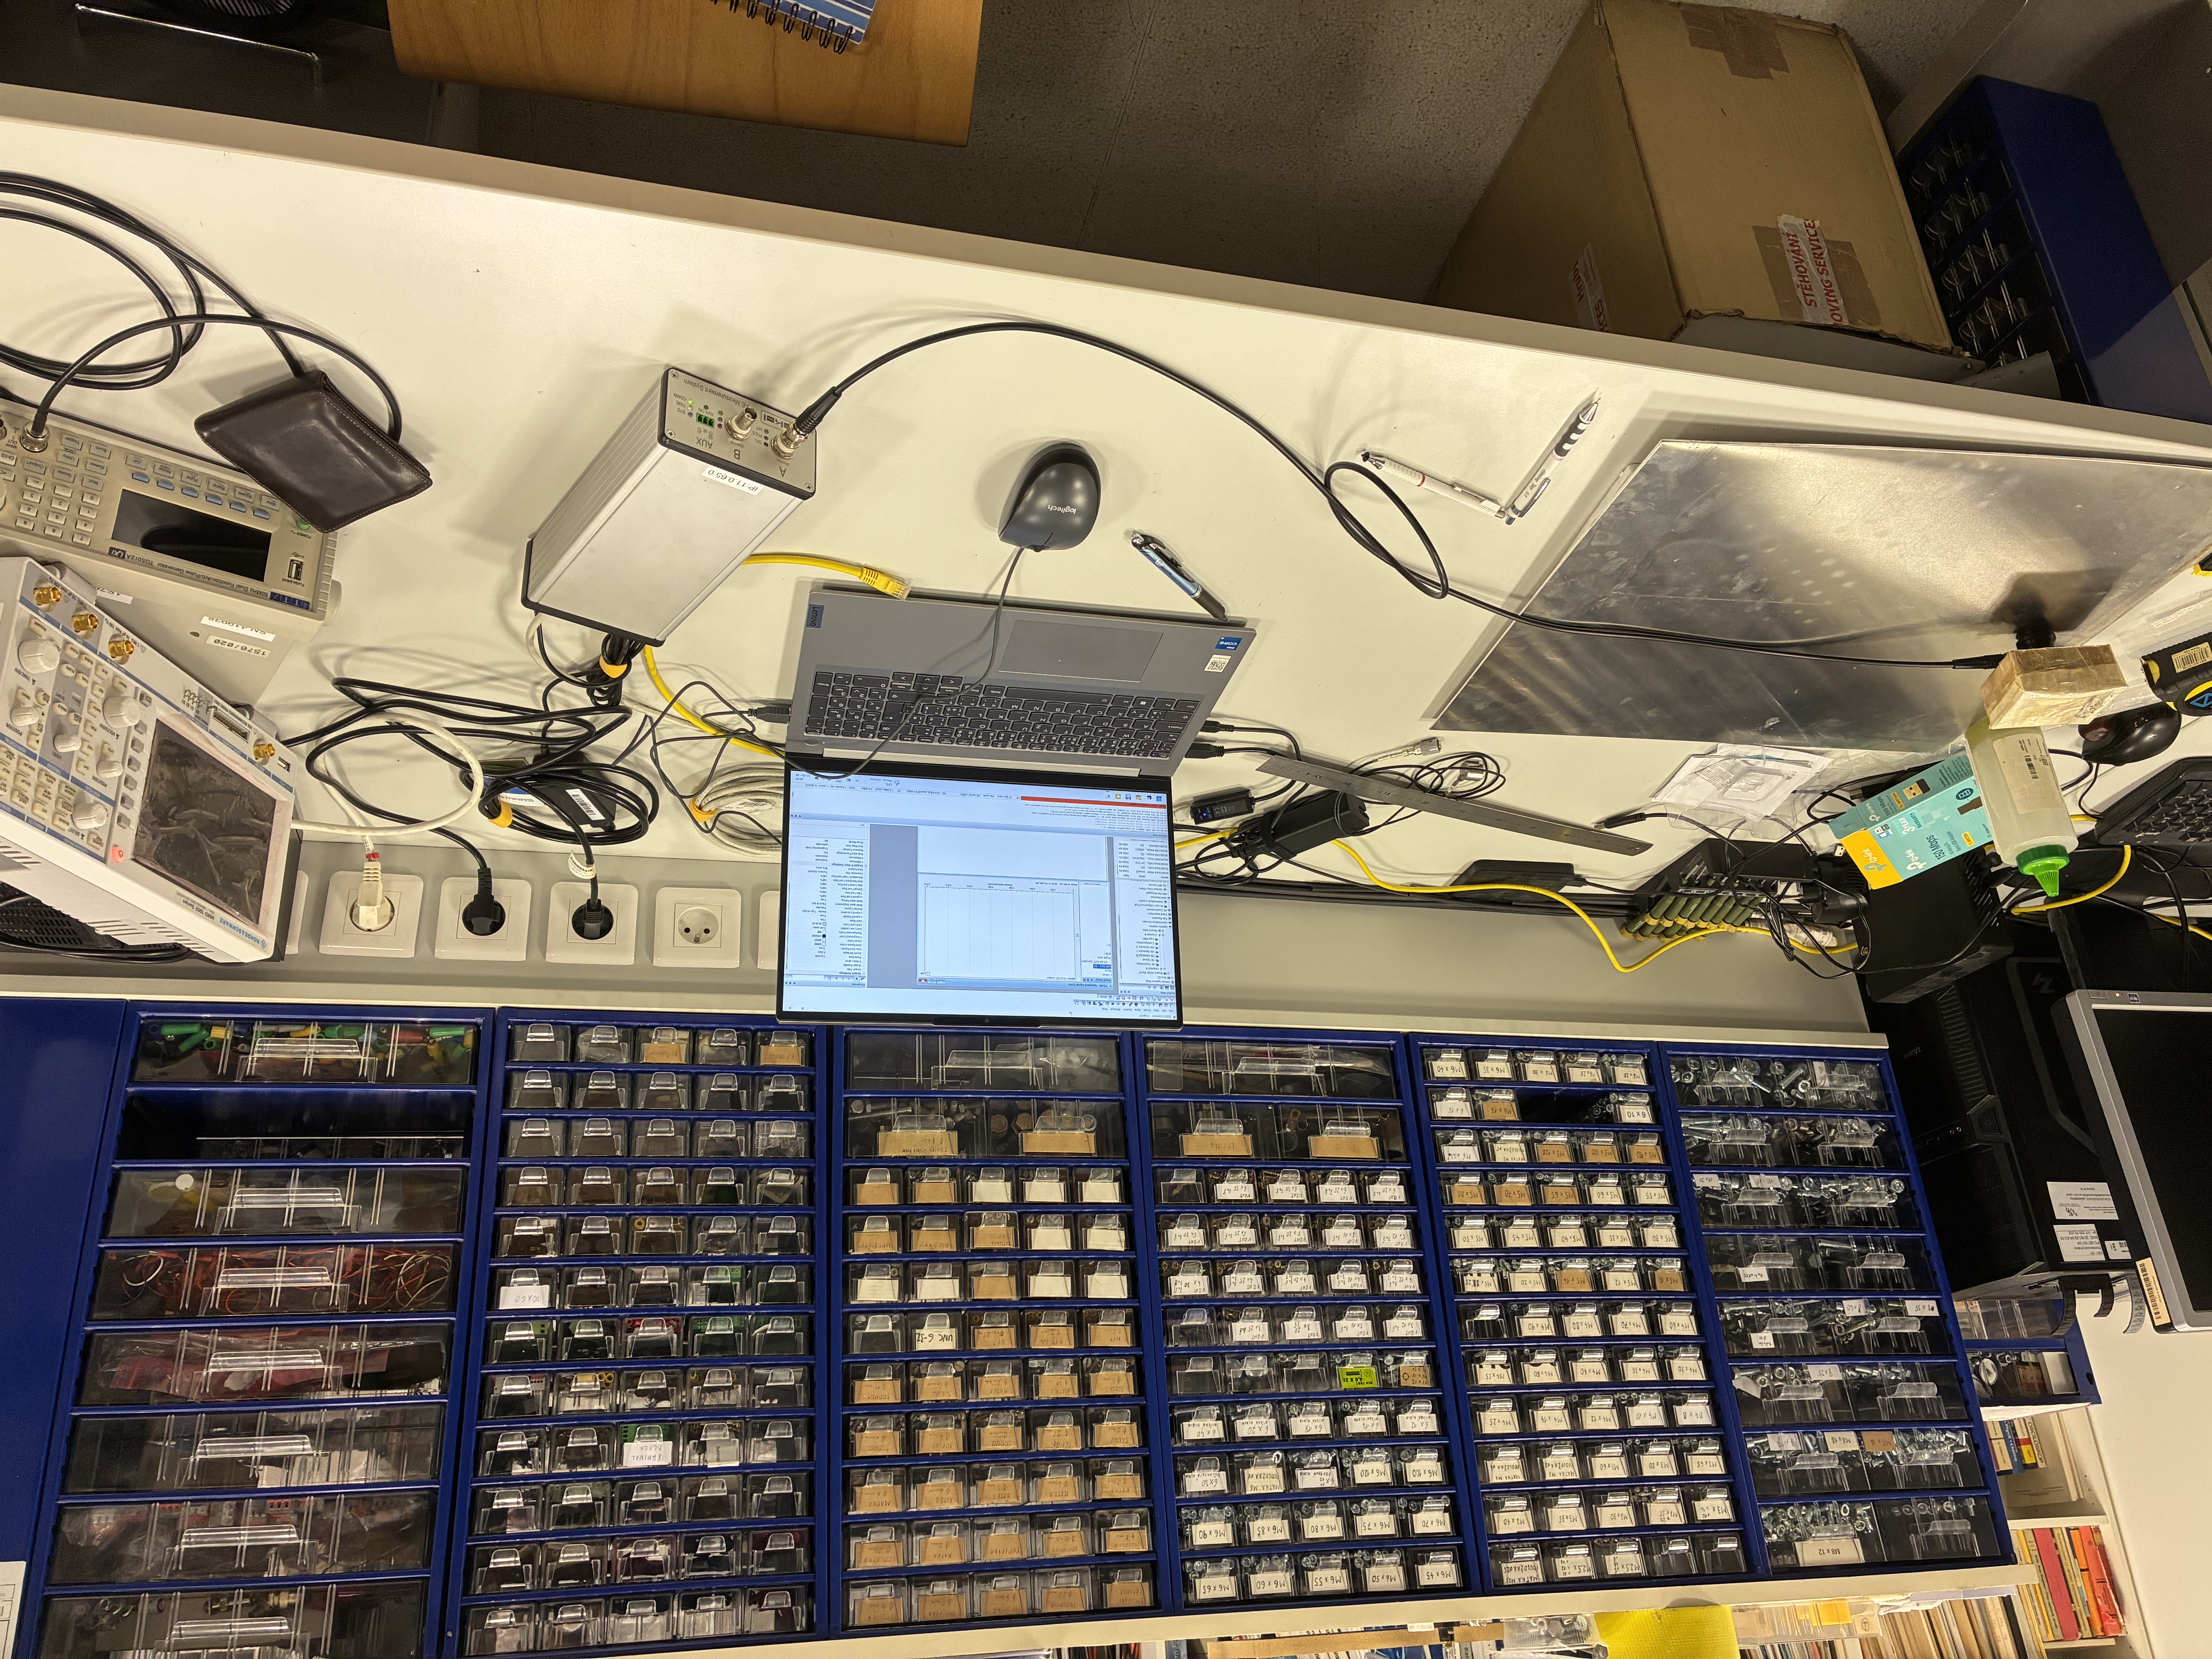
\includegraphics[angle= 180, width=0.75\linewidth]{obrazky/pracoviste_dakel.jpg}
    \caption{Měřicí pracoviště}
    \label{fig:dakel_pracoviste}
\end{figure}







